% Source: Weinberg GR, physical PDF pp. 298--307 (printed pp. 276--285).
% Coverage: Section 10.7, Detection of Gravitational Radiation; equations
%           (10.7.1)--(10.7.19), including the unnumbered resonance formulas.
% Figures/tables/footnotes: Figure 10.1; reference markers 1, 3, 12--22.
% Status: source-reviewed and compile-clean.
% Uncertainties: none.

\subsection{Detection of Gravitational Radiation}\label{sec:10.7}

Experiments that aim at the detection of gravitational radiation have been
carried out by Weber over the last decade,%
\hyperref[ch10-ref-1]{\textsuperscript{1}}
and are presently being planned in laboratories throughout the world. Most of
these experiments make use of \emph{resonant quadrupole antennas}, which can be
any ``small'' mechanical or hydrodynamical system with a natural mode of free
oscillation. It happens that the effective cross-sections of these antennas can
be evaluated by use of the optical theorem derived in the last section, without
any need for a detailed analysis of the interaction between the gravitational
wave and the antenna.

Our first assumption is that the antenna is much smaller than the wavelength
\(2\pi/\omega\), so that the scattered gravitational wave is pure quadrupole
radiation. By the same reasoning that earlier led to
Eqs.~\eqref{eq:10.4.10}, \eqref{eq:10.4.12}, \eqref{eq:10.5.3}, and
\eqref{eq:10.5.4}, we may now conclude that the scattering amplitude in
Eq.~\eqref{eq:10.6.1} takes the form
\begin{equation}
  f_{\mu\nu}(\widehat{\mathbf{x}})
  =
  t_{\mu\nu}(\widehat{\mathbf{x}})
  -\frac12\eta_{\mu\nu}
  t^\lambda{}_\lambda(\widehat{\mathbf{x}}),
  \tag{10.7.1}\label{eq:10.7.1}
\end{equation}
where \(t_{\mu\nu}\) is proportional to the Fourier transform of the
perturbation in \(T_{\mu\nu}\) caused by the wave. Conservation of energy and
momentum gives, as before,
\begin{equation}
  t_{0\ii}(\widehat{\mathbf{x}})
  =
  -\widehat x^{\,j}t_{ji},
  \qquad
  t_{00}(\widehat{\mathbf{x}})
  =
  \widehat x^{\,\ii}\widehat x^{\,j}t_{ij},
  \tag{10.7.2}\label{eq:10.7.2}
\end{equation}
where \(t_{ij}\) is independent of \(\widehat{\mathbf{x}}\), though depending
of course on \(\omega\), \(e_{\mu\nu}\), and on the detailed interaction
between the incident wave and the antenna. Adopting a coordinate system in
which the incident propagation vector \(\mathbf{k}\) is in the 3-direction,
and a gauge in which the only nonvanishing elements of the polarization tensor
are \(e_{11}=-e_{22}\) and \(e_{12}=e_{21}\), the total cross-section
\eqref{eq:10.6.15} is now
\begin{equation}
  \sigma_{\mathrm{tot}}
  =
  \frac{
    2\pi\operatorname{Im}\!\left\{
      e_{11}^*(t_{11}-t_{22})+2e_{12}^*t_{12}
    \right\}
  }{
    \omega\left(\lvert e_{11}\rvert^2+\lvert e_{12}\rvert^2\right)
  }.
  \tag{10.7.3}\label{eq:10.7.3}
\end{equation}
Also, the angular integral in \eqref{eq:10.6.12} can now be calculated by the
same method as in Section~\ref{sec:10.5}, and we find for the elastic
scattering cross-section
\begin{equation}
  \sigma_{\mathrm{scat}}
  =
  \frac{
    4\pi\left[
      t_{ij}^*t_{ij}-\frac13\lvert t_{ii}\rvert^2
    \right]
  }{
    5\left(\lvert e_{11}\rvert^2+\lvert e_{12}\rvert^2\right)
  }.
  \tag{10.7.4}\label{eq:10.7.4}
\end{equation}

Our other assumption is that the scattering is resonant; that is, the
frequency \(\omega\) of the incident wave is close to a natural frequency
\(\omega_0\) of free oscillation of the antenna system. We can think of the
incident wave as merely serving to excite this free oscillation, which then
loses energy through reradiation of gravitational waves or into other channels,
corresponding to elastic scattering or to absorption of the incident wave,
respectively.

One consequence of this assumption is that the ratio of the elastic-scattering
cross-section to the total cross-section is simply equal to the fraction
\(\eta\) of the energy of the free oscillation that is dissipated as
gravitational radiation rather than heat, light, and so on:
\begin{equation}
  \sigma_{\mathrm{scat}}=\eta\sigma_{\mathrm{tot}},
  \tag{10.7.5}\label{eq:10.7.5}
\end{equation}
where
\[
  \eta\equiv\frac{\Gamma_{\mathrm{grav}}}{\Gamma},
\]
with \(\Gamma\) the total decay rate of the free oscillation and
\(\Gamma_{\mathrm{grav}}\) the decay rate owing to the emission of gravitational
radiation. Since \(\eta\) is a parameter characterizing the free oscillation of
the antenna, and has nothing to do with how the oscillation is excited, it is
independent of \(e_{\mu\nu}\).

Another consequence of resonant scattering is that the \emph{form} of the
matrix \(t_{ij}\) is given by some fixed matrix \(n_{ij}\), depending only on
the geometric properties of the oscillation being excited. That is,
\(t_{ij}\) must equal \(n_{ij}\) times some function of the polarization
components \(e_{11}\) and \(e_{12}\). The incident field is assumed here to be
weak, so this latter function must be linear, and therefore
\begin{equation}
  t_{ij}=n_{ij}(\alpha e_{11}+\beta e_{12}),
  \tag{10.7.6}\label{eq:10.7.6}
\end{equation}
with \(n_{ij}\), \(\alpha\), and \(\beta\) all independent of \(e_{11}\) and
\(e_{12}\). For instance, if the antenna has an axis of symmetry along some
direction \(\mathbf{n}\), then \(n_{ij}\) is a linear combination of
\(\delta_{ij}\) and \(n_i n_j\). The term proportional to \(\delta_{ij}\)
does not contribute to \eqref{eq:10.7.3} or \eqref{eq:10.7.4}, so in this
case we could take
\begin{equation}
  n_{ij}=n_i n_j.
  \tag{10.7.7}\label{eq:10.7.7}
\end{equation}

The two requirements \eqref{eq:10.7.5} and \eqref{eq:10.7.6} impose
stringent conditions on the scattering amplitude. Using
\eqref{eq:10.7.3}, \eqref{eq:10.7.4}, and \eqref{eq:10.7.6} in
\eqref{eq:10.7.5}, we find
\[
  \begin{split}
  &\frac{\eta}{\omega}
  \operatorname{Im}\!\left\{
    \left[
      e_{11}^*(n_{11}-n_{22})+2e_{12}^*n_{12}
    \right]
    (\alpha e_{11}+\beta e_{12})
  \right\}
  \\
  &\qquad
  =
  \frac25
  \lvert\alpha e_{11}+\beta e_{12}\rvert^2
  \left[
    n_{ij}^*n_{ij}-\frac13\lvert n_{ii}\rvert^2
  \right].
  \end{split}
\]
This must hold for all \(e_{\mu\nu}\), so by equating the coefficients of
\(\lvert e_{11}\rvert^2\), \(e_{11}^*e_{12}\), and
\(\lvert e_{12}\rvert^2\), we obtain
\[
  \begin{split}
  \frac{1}{\lvert\alpha\rvert^2}
  \operatorname{Im}\!\left\{(n_{11}-n_{22})\alpha\right\}
  &=
  \frac{1}{2\alpha^*\beta}
  \left\{
    (n_{11}-n_{22})\beta-2n_{12}\alpha^*
  \right\}
  \\
  &=
  \frac{2}{\lvert\beta\rvert^2}
  \operatorname{Im}\!\left\{n_{12}\beta\right\}
  \\
  &=
  \frac{2\omega}{5\eta}
  \left[
    n_{ij}^*n_{ij}-\frac13\lvert n_{ii}\rvert^2
  \right].
  \end{split}
\]
The solution of these equations takes the form
\[
  \alpha
  =
  \frac{
    5\eta g(n_{11}^*-n_{22}^*)
  }{
    2\omega\left[
      n_{ij}^*n_{ij}-\frac13\lvert n_{ii}\rvert^2
    \right]
  },
\]
\[
  \beta
  =
  -\frac{
    5\eta g n_{12}^*
  }{
    \omega\left[
      n_{ij}^*n_{ij}-\frac13\lvert n_{ii}\rvert^2
    \right]
  },
\]
where \(g\) is a complex number with
\begin{equation}
  \operatorname{Im}g=\lvert g\rvert^2.
  \tag{10.7.8}\label{eq:10.7.8}
\end{equation}
The scattering amplitude \eqref{eq:10.7.6} is now
\begin{equation}
  t_{ij}
  =
  \frac{
    5g\eta n_{ij}
    \left[
      (n_{11}^*-n_{22}^*)e_{11}+2n_{12}^*e_{12}
    \right]
  }{
    2\omega\left[
      n_{lm}^*n_{lm}-\frac13\lvert n_{ll}\rvert^2
    \right]
  }.
  \tag{10.7.9}\label{eq:10.7.9}
\end{equation}
Note that this depends only on the form of the matrix \(n_{ij}\), not on its
normalization.

The final consequence of the assumption of resonant scattering is that the
frequency dependence of the scattering amplitude \(t_{ij}\) is given by the
Fourier transform of a function with time dependence
\[
  e^{-\ii\omega_0t}e^{-\Gamma t/2},
\]
which oscillates at frequency \(\omega_0\), and decays in amplitude and energy
at the rates \(\Gamma/2\) and \(\Gamma\), respectively. That is,
\(t_{ij}\) must have the frequency dependence
\begin{equation}
  t_{ij}\propto
  \left(\omega-\omega_0+\ii\frac{\Gamma}{2}\right)^{-1}.
  \tag{10.7.10}\label{eq:10.7.10}
\end{equation}
Since \(\eta\) and \(n_{ij}\) depend on the properties of the free oscillation,
and not on how it is produced, this frequency dependence can only arise from
the factor \(g\). In order to satisfy the ``unitarity'' condition
\eqref{eq:10.7.8} for all \(\omega\), we must then have
\begin{equation}
  g
  =
  \frac{-\Gamma/2}{\omega-\omega_0+\ii\Gamma/2}.
  \tag{10.7.11}\label{eq:10.7.11}
\end{equation}
The total cross-section \eqref{eq:10.7.3} for absorption or scattering of
gravitational waves by the antenna is then, in c.g.s.\ units,
\begin{equation}
  \begin{split}
  \sigma_{\mathrm{tot}}
  &=
  \left(\frac{5\pi\eta c^2}{\omega^2}\right)
  \left[
    \frac{\Gamma^2/4}
    {(\omega-\omega_0)^2+\Gamma^2/4}
  \right]
  \\
  &\quad\times
  \frac{
    \left|
      (n_{11}^*-n_{22}^*)e_{11}+2n_{12}^*e_{12}
    \right|^2
  }{
    \left[
      n_{ij}^*n_{ij}-\frac13\lvert n_{ii}\rvert^2
    \right]
    \left(
      \lvert e_{11}\rvert^2+\lvert e_{12}\rvert^2
    \right)
  }.
  \end{split}
  \tag{10.7.12}\label{eq:10.7.12}
\end{equation}
It is truly remarkable that this cross-section is entirely determined as a
function of \(e_{\mu\nu}\) and \(\omega\) by the parameters \(\omega_0\),
\(\Gamma\), and \(\eta\), and by the form of the matrix \(n_{ij}\), whether
the resonant oscillation is mechanical, acoustical, electrical, or anything
else.

In the special case of an antenna with an axis of circular symmetry
\(\mathbf{n}\), the matrix \(n_{ij}\) has the simple form
\eqref{eq:10.7.7}. Taking the symmetry axis to lie in the 1--3 plane at an
angle \(\theta\) to the incident 3-direction, the nonvanishing elements of
this matrix are
\[
  n_{11}=\sin^2\theta,
  \qquad
  n_{13}=\cos\theta\sin\theta,
  \qquad
  n_{33}=\cos^2\theta.
\]
The total cross-section \eqref{eq:10.7.12} is then
\begin{equation}
  \begin{split}
  \sigma_{\mathrm{tot}}
  &=
  \left(\frac{15\pi\eta c^2}{2\omega^2}\right)
  \left[
    \frac{\Gamma^2/4}
    {(\omega-\omega_0)^2+\Gamma^2/4}
  \right]
  \sin^4\theta
  \\
  &\quad\times
  \frac{\lvert e_{11}\rvert^2}
  {\lvert e_{11}\rvert^2+\lvert e_{12}\rvert^2}.
  \end{split}
  \tag{10.7.13}\label{eq:10.7.13}
\end{equation}
The factor \(\sin^4\theta\) makes the cross-section greatest when the antenna
axis is oriented at right angles to the direction of wave propagation, that
is, for \(\theta=\pi/2\). This is just a reflection of the fact that
gravitational waves, like electromagnetic waves, are \emph{transverse}.

When the polarization of the gravitational wave is not measured, the quantity
of interest is the average of \eqref{eq:10.7.12} over the helicities
\(\pm2\), that is, over polarization tensors with
\(e_{11}=\mp\ii e_{12}\):
\begin{equation}
  \overline{\sigma}_{\mathrm{tot}}
  =
  \left(\frac{5\pi\eta c^2}{2\omega^2}\right)
  \left[
    \frac{\Gamma^2/4}
    {(\omega-\omega_0)^2+\Gamma^2/4}
  \right]
  \frac{
    \lvert n_{11}-n_{22}\rvert^2+4\lvert n_{12}\rvert^2
  }{
    n_{ij}^*n_{ij}-\frac13\lvert n_{ii}\rvert^2
  }.
  \tag{10.7.14}\label{eq:10.7.14}
\end{equation}
For an antenna with an axis of circular symmetry, the effect of averaging over
helicities is just to replace the last factor in Eq.~\eqref{eq:10.7.13} with
\(1/2\).

The above analysis is strictly applicable only where there is a single
nondegenerate resonant oscillation. When there are several degenerate modes,
the particular linear combination excited by a gravitational wave can depend
on the polarization of the wave, so that \(t_{ij}\) need not be proportional
to a fixed matrix \(n_{ij}\). For instance, if the antenna is an elastic
sphere, then any quadrupole oscillation will consist of five independent
modes. In this case, \(t_{ij}\) must be a linear combination of
\(\delta_{ij}\) and \(e_{ij}\), but again the term proportional to
\(\delta_{ij}\) does not contribute to \eqref{eq:10.7.3} or
\eqref{eq:10.7.4}, so we can take
\[
  t_{ij}=\gamma e_{ij}.
\]
Equations \eqref{eq:10.7.3}--\eqref{eq:10.7.5} now give
\[
  \operatorname{Im}\gamma=\frac{2\omega}{5\eta}\lvert\gamma\rvert^2,
\]
so, since \(\gamma\) must have the frequency dependence
\eqref{eq:10.7.10}, it is
\[
  \gamma
  =
  \left(\frac{5\eta}{2\omega}\right)
  \left(
    \frac{-\Gamma/2}{\omega-\omega_0+\ii\Gamma/2}
  \right).
\]
The total cross-section \eqref{eq:10.7.3} is now
\begin{equation}
  \sigma_{\mathrm{tot}}
  =
  \left(\frac{10\pi\eta c^2}{\omega^2}\right)
  \left[
    \frac{\Gamma^2/4}
    {(\omega-\omega_0)^2+\Gamma^2/4}
  \right],
  \tag{10.7.15}\label{eq:10.7.15}
\end{equation}
for any incident polarization.

In all cases the effective cross-section has a maximum when the antenna is
\emph{tuned}, so that the resonant frequency \(\omega_0\) is equal to the
frequency \(\omega\) of the incident wave. Inspection of
\eqref{eq:10.7.12}--\eqref{eq:10.7.15} shows that this maximum
cross-section is of the order
\begin{equation}
  \sigma_{\max}\approx\eta\lambda^2,
  \tag{10.7.16}\label{eq:10.7.16}
\end{equation}
where \(\lambda\) is the wavelength \(2\pi c/\omega\). In the ideal case of
an oscillation that decays purely through the emission of gravitational
radiation, we would have \(\eta=1\), and \(\sigma_{\max}\) would have the
very large value \(\lambda^2\). Of course, this ideal case is never even
approached in practice; for instance, we found in Section~\ref{sec:10.5} that
Weber's large aluminum cylinders have
\(\eta\simeq3\times10^{-34}\). Generally, the rate \(\Gamma_{\mathrm{grav}}\)
at which a resonant oscillator emits gravitational radiation depends on the
gross dimensions of the antenna and is difficult to increase; thus, in order
to make \(\sigma_{\max}\) as large as possible, it is necessary to reduce the
total loss rate \(\Gamma\) in the ratio
\(\eta\equiv\Gamma_{\mathrm{grav}}/\Gamma\) as much as possible, possibly by
employing some sort of oscillation in a superfluid.

However, tuning our antenna does no good unless we have some strong source of
gravitational radiation with a known frequency to which we can tune. Perhaps
the most promising source%
\hyperref[ch10-ref-12]{\textsuperscript{12}}
is the pulsar NP~0532 in the Crab nebula. This object is observed to emit
pulses of electromagnetic radiation at optical, X-ray, and radio frequencies
with a period \(2\pi/\Omega=0.03309\,\mathrm{sec}\). As discussed in
Section~\ref{sec:10.5}, the pulsars are believed to be rotating neutron
stars%
\hyperref[ch10-ref-3]{\textsuperscript{3}}
with moments of inertia of order \(10^{45}\,\mathrm{g\,cm^2}\) and unknown
equatorial ellipticities \(e\). The Crab pulsar is therefore presumably
emitting gravitational radiation, with
\(\omega=2\Omega=379.8\,\mathrm{Hz}\), at a rate of about
\(10^{45}e^2\,\mathrm{ergs/sec}\). Since the Crab nebula is at a distance
of 6500 light-years, or \(6.2\times10^{21}\,\mathrm{cm}\), the flux of
gravitational radiation passing the earth should be about
\(\Phi\simeq e^2\,\mathrm{ergs/(sec\,cm^2)}\). A resonant linear quadrupole
antenna that is ``aimed'' at and tuned to the Crab pulsar will have a
cross-section \(\overline{\sigma}_{\mathrm{tot}}\) given by
\eqref{eq:10.7.13} as \(7.4\times10^{16}\eta\,\mathrm{cm^2}\). The power
absorbed by the antenna will thus be of order
\(10^{16}e^2\eta\,\mathrm{ergs/sec}\). For instance, if \(\eta\) is
\(10^{-32}\) and \(e\) is of order \(10^{-4}\), this power is of order
\(10^{-24}\,\mathrm{ergs/sec}\), which might perhaps be detectable.
Unfortunately, in order to use an aluminum cylinder of the sort discussed in
Section~\ref{sec:10.5} as an antenna tuned to the Crab, the cylinder would
have to have the rather ungainly length \(\pi v_s/\omega\) of 42 meters. To
get around this difficulty, one can use as antennas hoops, forks, and so on,
which have lower natural frequencies for a given size than bars or cylinders.
A group at Rochester%
\hyperref[ch10-ref-13]{\textsuperscript{13}}
is planning a hoop antenna that could be tuned to the Crab.

All of the experiments carried out so far by Weber have made use of resonant
quadrupole antennas that are \emph{not} tuned to any particular source. Since
it is too much to ask that a monochromatic source like a pulsar should just
happen to fall within the bandwidth of the antenna, these experiments really
aim at the detection of broadband gravitational radiation, with an energy flux
\(\Phi(\omega)\,\dd\omega\) between frequencies \(\omega\) and
\(\omega+\dd\omega\). If exposed to such radiation, the power absorbed by a
resonant antenna will be
\[
  P
  =
  \sigma_{\max}
  \int
  \frac{\Gamma^2/4}
  {(\omega-\omega_0)^2+\Gamma^2/4}
  \Phi(\omega)\,\dd\omega,
\]
where \(\sigma_{\max}\) is the effective cross-section of the antenna at
resonance, given by setting \(\omega=\omega_0\) in
\eqref{eq:10.7.12}, \eqref{eq:10.7.13}, \eqref{eq:10.7.14}, or
\eqref{eq:10.7.15}. If \(\Phi(\omega)\) is roughly constant over the
frequency range \(\omega_0-\Gamma\) to \(\omega_0+\Gamma\), then it can be
taken out of the integral, and we have
\begin{equation}
  P=\pi\sigma_{\max}\Phi(\omega_0)\frac{\Gamma}{2}.
  \tag{10.7.17}\label{eq:10.7.17}
\end{equation}

For a source that radiates for a time much longer than the antenna relaxation
time \(1/\Gamma\), a quasi-steady state will be reached in which the mean
energy \(E\) in the resonant mode is such that the loss rate \(E\Gamma\) just
balances the absorbed power \(P\):
\begin{equation}
  E
  =
  \frac{P}{\Gamma}
  =
  \pi\sigma_{\max}\frac{\Phi(\omega_0)}{2}.
  \tag{10.7.18}\label{eq:10.7.18}
\end{equation}
In this case, a measurement of the mean excitation energy of the resonant mode
serves to measure, or at least to set an upper limit on, the power flux at the
resonant frequency. For instance, the earth has a fundamental spheroidal
oscillation mode%
\hyperref[ch10-ref-14]{\textsuperscript{14}}
\({}_0S_2\), with a period \(2\pi/\omega\) of 54 min and a decay rate
\(\Gamma\) of order \(5\times10^{-6}\,\mathrm{sec^{-1}}\), in which the
mass-density perturbation is of the form
\(\rho_1(r)Y_2^m(\theta,\phi)\). The gravitational decay rate
\(\Gamma_{\mathrm{grav}}\) of this mode will be roughly of order
\(GM_\oplus R_\oplus^2\omega^4/c^5\), or about
\(10^{-25}\,\mathrm{sec^{-1}}\), so the branching ratio \(\eta\) is of
order \(10^{-20}\). The cross-section \eqref{eq:10.7.15} at resonance is
here \(7.5\times10^{27}\eta\,\mathrm{cm^2}\), or roughly
\(10^7\) to \(10^8\,\mathrm{cm^2}\). From seismic measurements of the
mean strain in the earth's crust during quiet periods, Forward et al.%
\hyperref[ch10-ref-15]{\textsuperscript{15}}
in 1961 set an upper limit on \(\Phi(\omega_0)\) of roughly
\(20\,\mathrm{watts/(cm^2\,Hz)}\). It is hoped that a much better upper
limit on \(\Phi\) can be set by placing a gravimeter on the moon,%
\hyperref[ch10-ref-16]{\textsuperscript{16}}
which is very much quieter seismically than the earth.

For a ``burst'' source that radiates for a time \(\tau\) less than the antenna
relaxation time \(1/\Gamma\), the total energy picked up by the antenna will
be
\[
  \Delta E
  =
  P\tau
  =
  \pi\sigma_{\max}\Phi(\omega_0)\tau\frac{\Gamma}{2}.
\]
Thus the energy per unit area in the burst reaching the antenna
\emph{within the beam width} \(\Gamma\) may be determined as
\begin{equation}
  \mathcal{E}
  \equiv
  \Phi(\omega_0)\Gamma\tau
  =
  \frac{2\Delta E}{\pi\sigma_{\max}}.
  \tag{10.7.19}\label{eq:10.7.19}
\end{equation}
However, if the source radiates for a time \(\tau<1/\Gamma\), its bandwidth
must be greater than \(1/\tau\), so the \emph{total} energy per unit area in
the burst must be larger than \(\mathcal{E}\) by a factor greater than
\((\tau\Gamma)^{-1}\).

The only positive indication so far of the presence of gravitational radiation
in the universe comes from the experiments of Weber,%
\hyperref[ch10-ref-1]{\textsuperscript{1}}
which use as antennas the aluminum cylinders described in
Section~\ref{sec:10.5}. These antennas have the frequency and ``branching
ratio''
\[
  \frac{\omega_0}{2\pi}=1660\,\mathrm{Hz},
  \qquad
  \eta=3\times10^{-34}.
\]
By setting \(\omega=\omega_0\) and averaging over helicities in
Eq.~\eqref{eq:10.7.13}, we find a cross-section at resonance
\[
  \overline{\sigma}_{\max}
  =
  2.9\times10^{-20}\sin^4\theta\;\mathrm{cm^2}.
\]
If the smallest energy increment \(\Delta E\) that can be distinguished from
thermal fluctuations is \(kT\), or \(4\times10^{-14}\) ergs at room
temperature, then according to \eqref{eq:10.7.19}, a burst of gravitational
radiation will be detectable if the energy \(\mathcal{E}\) per unit area
within the beam width satisfies
\[
  \mathcal{E}\gtrsim9\times10^5\,\mathrm{ergs/cm^2}
  \qquad\text{for}\qquad
  \theta=\frac{\pi}{2}.
\]
(It is actually possible to do a little better than this by careful data
processing.) The mere observation of a number of pulses in a single cylinder
would leave open the possibility that these pulses were due to nonthermal
noise, such as seismic disturbances, electric storms, or cosmic rays, so Weber
looked for coincident pulses in aluminum cylinders 1000 km apart, at College
Park in Maryland and the Argonne National Laboratory in Illinois. In 1969
Weber reported over 100 coincident pulses, occurring at a rate that indicates
a mean gravitational-radiation flux, within the bandwidth
\(\Gamma\sim0.1\,\mathrm{Hz}\), of about
\(0.1\,\mathrm{erg\,cm^{-2}\,sec^{-1}}\).%
\hyperref[ch10-ref-17]{\textsuperscript{17}}

Shortly thereafter,%
\hyperref[ch10-ref-18]{\textsuperscript{18}}
Weber found that the rate of coincident pulses was correlated with sidereal
time, in a manner consistent with the expected \(\sin^4\theta\) antenna
pattern if the gravitational radiation is coming from the center of our galaxy
(see Figure~\ref{fig:10.1}). The galactic center is about
\(2.5\times10^{22}\,\mathrm{cm}\) from the earth, so an observed flux of
\(0.1\,\mathrm{erg\,cm^{-2}\,sec^{-1}}\) would indicate an energy
production of about \(8\times10^{44}\,\mathrm{ergs/sec}\), or
\(0.013M_\odot c^2/\mathrm{year}\). This would not in itself be so
remarkable, but since Weber's antennas are not tuned to any particular
frequency, an energy production of \(0.01M_\odot c^2\) in a bandwidth of
0.1 Hz at 1660 Hz presumably represents a total energy production \(10^3\)
to \(10^5\) times larger, or \(10\) to \(10^3M_\odot c^2/\mathrm{year}\).
At this rate, the whole mass of the galaxy would be used up in \(10^8\) to
\(10^{10}\) years. If Weber is really observing gravitational radiation from
the galactic center, then either he accidentally picked the precise frequency
at which most of this radiation is emitted, or else he has discovered an
incredibly powerful new source of energy.

Weber has also looked for scalar radiation, using a disk with a monopole mode
of oscillation having the same frequency, 1660 Hz, as the cylinders. The
coincidence rate is observed to be much less than for the pair of cylinders;
the apparent correlation of coincidences with sidereal time agrees with a pure
tensor theory.%
\hyperref[ch10-ref-19]{\textsuperscript{19}}

% Source: Weinberg GR, physical PDF p. 306 (printed p. 284).
% Coverage: Figure 10.1, Weber detector intensity versus sidereal time.
% Status: source plot extracted at high resolution; source-reviewed and
%         compile-clean.
% Uncertainties: none.

\begingroup
\renewcommand{\thefigure}{10.1}
\begin{figure}[t]
\centering
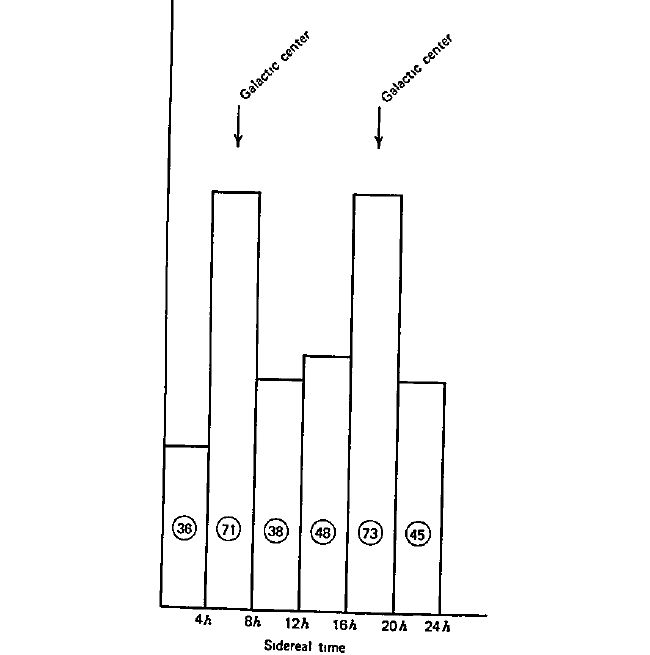
\includegraphics[width=0.76\textwidth]{figures/chapter10/fig10-01.png}
\caption{Evidence for gravitational radiation emanating from the center of
the galaxy.\hyperref[ch10-ref-18]{\textsuperscript{18}} The detector
intensity observed by Weber is plotted here (in arbitrary units) against
sidereal time. Arrows mark the sidereal times at which the antenna is most
nearly perpendicular to the line of sight to the center of the galaxy.
Numbers in circles are the observed numbers of coincidences in each time
interval.}
\label{fig:10.1}
\end{figure}
\endgroup


Plans are now in train to repeat Weber's experiments with much greater
sensitivity. One important improvement that is being planned at Stanford%
\hyperref[ch10-ref-20]{\textsuperscript{20}}
is to operate a cylindrical antenna at a very low temperature, in the range of
millidegrees Kelvin. If the antenna is limited by thermal noise, then lowering
the temperature by a factor \(10^{-3}\) would increase the sensitivity by a
factor \(10^3\). A group at Moscow%
\hyperref[ch10-ref-21]{\textsuperscript{21}}
is carrying out gravitational-radiation experiments with improved
instrumentation, and is designing novel kinds of gravitational-wave
antennas.%
\hyperref[ch10-ref-22]{\textsuperscript{22}}
Weber is continuing his observations, using new antennas and instrumentation.
At present, the best a theorist can do is to wait for the experimentalists to
reach some sort of consensus on whether gravitational radiation has indeed
been observed.
